\section{Data}\label{sec:data}

We used two datasets with the same patch format: EuroSAT to train the models in Europe, and a
new set of labeled patches from Aguascalientes to fine-tune and test them. We kept the format
identical so that the main thing that changes between the two is the landscape.

\subsection{EuroSAT}

We used EuroSAT~\cite{helber2019eurosat}, a dataset of Sentinel-2
images in 13 spectral bands and 10 land-use classes. Its multispectral version, EuroSAT MS, holds
L1C patches of 13$\times$64$\times$64 pixels at 10~m. We kept the official TorchGeo split of \num{16200} training,
\num{5400} validation and \num{5400} test patches, and the TorchGeo band order (B01 to B12, with B8A last).
The RGB input is B04, B03 and B02 taken from the same 13-band files. We chose this so that the
RGB and 13-band runs see the same patches and the same pixel values; only the number of bands
changes. With a separately processed RGB version, part of any gap between the two inputs could
come from that processing instead of from the bands.

\subsection{Aguascalientes composite and grid}

We built one Sentinel-2 composite of the state for April 2024 in Google Earth Engine. We used
the L1C harmonized collection (\texttt{COPERNICUS/S2\_HARMONIZED}, digital numbers equal to
reflectance $\times$ \num{10000}) because EuroSAT is also L1C. With surface reflectance (L2A), the
models would face a change of processing level on top of the change of region. We chose April
because it falls in the dry season, and March and April are the months with the least rain of
the year~\cite{inagua2022planhidrico}, so one month gives enough clear images. Clouds were
masked with QA60 bits 10 (opaque) and 11 (cirrus), and we took the per-pixel median of the month.
The median reduces the clouds and shadows that the mask misses, because they are outliers in the
time series of each pixel. All bands were resampled to 10~m and clipped to the state boundary
of FAO GAUL 2025 level~1.

We cut the composite with an absolute 640~m grid in EPSG:32613 and extracted one
13$\times$64$\times$64 patch per cell, in the EuroSAT band order. The grid size follows from
EuroSAT: 64~pixels of 10~m cover 640~m, so each cell is exactly one EuroSAT-sized patch. The grid
origin lies on multiples of 640~m, so no pixel is split between two cells.

\subsection{Labels and spatial split}

A single annotator labeled the cells with the 10 EuroSAT classes on an RGB preview of the
composite. The April 2024 preview was the main evidence; the Esri World Imagery basemap was used
only to recognize objects such as roofs, tree rows and roads, because it is recent imagery,
often from another season. A cell got a class only if at least 70\,\% of it was that class; Highway and River
were labeled by their dominant element. A labeling guide fixed tie-breakers for
semi-arid confusions: xeric scrub is HerbaceousVegetation, managed grazing grass is Pasture,
continuous canopy is Forest, and trees or vines in rows are PermanentCrop. We refined the guide
after the first 547 cells and re-labeled those cells with the final version (details in the
data card). Cells whose cover has
no EuroSAT class (greenhouses, quarries, bare rock or soil) or that raised any doubt were
skipped and never used. This reduces label noise in the test set, but it also means the test
set does not measure errors on those covers.

Neighboring cells are almost identical, so we split by space and not by cell. A random cell
split would put near-duplicates in the fine-tune and test sets and inflate the scores. Instead,
we grouped the cells into blocks of 8$\times$8 cells (5.12~km), and each block went whole to
one split. With seed 0, we shuffled the block list \num{20000} times, cut it half/half, and kept the
partition with the smallest maximum deviation of any class from 50\,\% in test. That deviation
was 0.0294, so every class is split almost evenly; each split holds 119 blocks. The split has
no buffer zone, which leaves a residual risk: 35 of the 541 test patches border a fine-tune
cell across a block edge, so the fine-tuned scores may be slightly optimistic.

Table~\ref{tab:ags_classes} lists the labeled patches per class and split. It shows a strong
imbalance: HerbaceousVegetation has 236 test patches and SeaLake only 13. River has 7, fewer
than 10, so we left it out of the Aguascalientes macro-F1 and report it separately. The last row
counts the 168 skipped cells, which appear in no experiment.
Fig.~\ref{fig:study_area} shows the blocks on the composite and compares patches of the same
class from both regions. The gap is visible before any model is trained.

\begin{table}[t]
\centering
\footnotesize
\caption{Labeled Aguascalientes patches per class and split. $^\dagger$Fewer than 10 test patches: left out of the Aguascalientes macro-F1 and reported separately.}
\label{tab:ags_classes}
\begin{tabular}{@{}lrrr@{}}
\toprule
Class & Fine-tune & Test & Total \\
\midrule
AnnualCrop & \num{109} & \num{104} & \num{213} \\
Forest & \num{45} & \num{40} & \num{85} \\
HerbaceousVegetation & \num{245} & \num{236} & \num{481} \\
Highway & \num{33} & \num{31} & \num{64} \\
Industrial & \num{24} & \num{24} & \num{48} \\
Pasture & \num{24} & \num{26} & \num{50} \\
PermanentCrop & \num{24} & \num{26} & \num{50} \\
Residential & \num{38} & \num{34} & \num{72} \\
River$^\dagger$ & \num{7} & \num{7} & \num{14} \\
SeaLake & \num{12} & \num{13} & \num{25} \\
\midrule
Total labeled & \num{561} & \num{541} & \num{1102} \\
Skipped (not used) & \num{85} & \num{83} & \num{168} \\
\bottomrule
\end{tabular}
\end{table}


\begin{figure}[t]
\centering
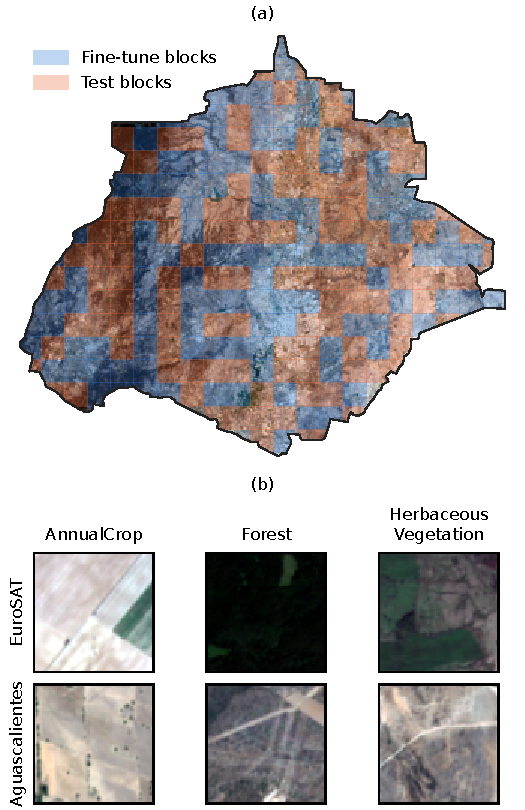
\includegraphics[width=\columnwidth]{study_area}
\caption{(a) April 2024 RGB composite of Aguascalientes with the 8$\times$8-cell blocks colored
by split (blue: fine-tune, orange: test) and the state outline. (b) One EuroSAT test patch (top
row) and one Aguascalientes test patch (bottom row) for AnnualCrop, Forest and
HerbaceousVegetation; they are the patches of the Grad-CAM figures. RGB stretch 2--98\,\% per
dataset; Aguascalientes uses the global limits of the composite, as the labeling previews did.
Note how differently the same class looks in Europe and in semi-arid Aguascalientes.}
\label{fig:study_area}
\end{figure}
